% Options for packages loaded elsewhere
\PassOptionsToPackage{unicode}{hyperref}
\PassOptionsToPackage{hyphens}{url}
\PassOptionsToPackage{dvipsnames,svgnames,x11names}{xcolor}
%
\documentclass[
  letterpaper,
  DIV=11,
  numbers=noendperiod]{scrartcl}

\usepackage{amsmath,amssymb}
\usepackage{iftex}
\ifPDFTeX
  \usepackage[T1]{fontenc}
  \usepackage[utf8]{inputenc}
  \usepackage{textcomp} % provide euro and other symbols
\else % if luatex or xetex
  \usepackage{unicode-math}
  \defaultfontfeatures{Scale=MatchLowercase}
  \defaultfontfeatures[\rmfamily]{Ligatures=TeX,Scale=1}
\fi
\usepackage{lmodern}
\ifPDFTeX\else  
    % xetex/luatex font selection
\fi
% Use upquote if available, for straight quotes in verbatim environments
\IfFileExists{upquote.sty}{\usepackage{upquote}}{}
\IfFileExists{microtype.sty}{% use microtype if available
  \usepackage[]{microtype}
  \UseMicrotypeSet[protrusion]{basicmath} % disable protrusion for tt fonts
}{}
\makeatletter
\@ifundefined{KOMAClassName}{% if non-KOMA class
  \IfFileExists{parskip.sty}{%
    \usepackage{parskip}
  }{% else
    \setlength{\parindent}{0pt}
    \setlength{\parskip}{6pt plus 2pt minus 1pt}}
}{% if KOMA class
  \KOMAoptions{parskip=half}}
\makeatother
\usepackage{xcolor}
\setlength{\emergencystretch}{3em} % prevent overfull lines
\setcounter{secnumdepth}{-\maxdimen} % remove section numbering
% Make \paragraph and \subparagraph free-standing
\makeatletter
\ifx\paragraph\undefined\else
  \let\oldparagraph\paragraph
  \renewcommand{\paragraph}{
    \@ifstar
      \xxxParagraphStar
      \xxxParagraphNoStar
  }
  \newcommand{\xxxParagraphStar}[1]{\oldparagraph*{#1}\mbox{}}
  \newcommand{\xxxParagraphNoStar}[1]{\oldparagraph{#1}\mbox{}}
\fi
\ifx\subparagraph\undefined\else
  \let\oldsubparagraph\subparagraph
  \renewcommand{\subparagraph}{
    \@ifstar
      \xxxSubParagraphStar
      \xxxSubParagraphNoStar
  }
  \newcommand{\xxxSubParagraphStar}[1]{\oldsubparagraph*{#1}\mbox{}}
  \newcommand{\xxxSubParagraphNoStar}[1]{\oldsubparagraph{#1}\mbox{}}
\fi
\makeatother

\usepackage{color}
\usepackage{fancyvrb}
\newcommand{\VerbBar}{|}
\newcommand{\VERB}{\Verb[commandchars=\\\{\}]}
\DefineVerbatimEnvironment{Highlighting}{Verbatim}{commandchars=\\\{\}}
% Add ',fontsize=\small' for more characters per line
\usepackage{framed}
\definecolor{shadecolor}{RGB}{241,243,245}
\newenvironment{Shaded}{\begin{snugshade}}{\end{snugshade}}
\newcommand{\AlertTok}[1]{\textcolor[rgb]{0.68,0.00,0.00}{#1}}
\newcommand{\AnnotationTok}[1]{\textcolor[rgb]{0.37,0.37,0.37}{#1}}
\newcommand{\AttributeTok}[1]{\textcolor[rgb]{0.40,0.45,0.13}{#1}}
\newcommand{\BaseNTok}[1]{\textcolor[rgb]{0.68,0.00,0.00}{#1}}
\newcommand{\BuiltInTok}[1]{\textcolor[rgb]{0.00,0.23,0.31}{#1}}
\newcommand{\CharTok}[1]{\textcolor[rgb]{0.13,0.47,0.30}{#1}}
\newcommand{\CommentTok}[1]{\textcolor[rgb]{0.37,0.37,0.37}{#1}}
\newcommand{\CommentVarTok}[1]{\textcolor[rgb]{0.37,0.37,0.37}{\textit{#1}}}
\newcommand{\ConstantTok}[1]{\textcolor[rgb]{0.56,0.35,0.01}{#1}}
\newcommand{\ControlFlowTok}[1]{\textcolor[rgb]{0.00,0.23,0.31}{\textbf{#1}}}
\newcommand{\DataTypeTok}[1]{\textcolor[rgb]{0.68,0.00,0.00}{#1}}
\newcommand{\DecValTok}[1]{\textcolor[rgb]{0.68,0.00,0.00}{#1}}
\newcommand{\DocumentationTok}[1]{\textcolor[rgb]{0.37,0.37,0.37}{\textit{#1}}}
\newcommand{\ErrorTok}[1]{\textcolor[rgb]{0.68,0.00,0.00}{#1}}
\newcommand{\ExtensionTok}[1]{\textcolor[rgb]{0.00,0.23,0.31}{#1}}
\newcommand{\FloatTok}[1]{\textcolor[rgb]{0.68,0.00,0.00}{#1}}
\newcommand{\FunctionTok}[1]{\textcolor[rgb]{0.28,0.35,0.67}{#1}}
\newcommand{\ImportTok}[1]{\textcolor[rgb]{0.00,0.46,0.62}{#1}}
\newcommand{\InformationTok}[1]{\textcolor[rgb]{0.37,0.37,0.37}{#1}}
\newcommand{\KeywordTok}[1]{\textcolor[rgb]{0.00,0.23,0.31}{\textbf{#1}}}
\newcommand{\NormalTok}[1]{\textcolor[rgb]{0.00,0.23,0.31}{#1}}
\newcommand{\OperatorTok}[1]{\textcolor[rgb]{0.37,0.37,0.37}{#1}}
\newcommand{\OtherTok}[1]{\textcolor[rgb]{0.00,0.23,0.31}{#1}}
\newcommand{\PreprocessorTok}[1]{\textcolor[rgb]{0.68,0.00,0.00}{#1}}
\newcommand{\RegionMarkerTok}[1]{\textcolor[rgb]{0.00,0.23,0.31}{#1}}
\newcommand{\SpecialCharTok}[1]{\textcolor[rgb]{0.37,0.37,0.37}{#1}}
\newcommand{\SpecialStringTok}[1]{\textcolor[rgb]{0.13,0.47,0.30}{#1}}
\newcommand{\StringTok}[1]{\textcolor[rgb]{0.13,0.47,0.30}{#1}}
\newcommand{\VariableTok}[1]{\textcolor[rgb]{0.07,0.07,0.07}{#1}}
\newcommand{\VerbatimStringTok}[1]{\textcolor[rgb]{0.13,0.47,0.30}{#1}}
\newcommand{\WarningTok}[1]{\textcolor[rgb]{0.37,0.37,0.37}{\textit{#1}}}

\providecommand{\tightlist}{%
  \setlength{\itemsep}{0pt}\setlength{\parskip}{0pt}}\usepackage{longtable,booktabs,array}
\usepackage{calc} % for calculating minipage widths
% Correct order of tables after \paragraph or \subparagraph
\usepackage{etoolbox}
\makeatletter
\patchcmd\longtable{\par}{\if@noskipsec\mbox{}\fi\par}{}{}
\makeatother
% Allow footnotes in longtable head/foot
\IfFileExists{footnotehyper.sty}{\usepackage{footnotehyper}}{\usepackage{footnote}}
\makesavenoteenv{longtable}
\usepackage{graphicx}
\makeatletter
\def\maxwidth{\ifdim\Gin@nat@width>\linewidth\linewidth\else\Gin@nat@width\fi}
\def\maxheight{\ifdim\Gin@nat@height>\textheight\textheight\else\Gin@nat@height\fi}
\makeatother
% Scale images if necessary, so that they will not overflow the page
% margins by default, and it is still possible to overwrite the defaults
% using explicit options in \includegraphics[width, height, ...]{}
\setkeys{Gin}{width=\maxwidth,height=\maxheight,keepaspectratio}
% Set default figure placement to htbp
\makeatletter
\def\fps@figure{htbp}
\makeatother

\KOMAoption{captions}{tableheading}
\makeatletter
\@ifpackageloaded{caption}{}{\usepackage{caption}}
\AtBeginDocument{%
\ifdefined\contentsname
  \renewcommand*\contentsname{Table of contents}
\else
  \newcommand\contentsname{Table of contents}
\fi
\ifdefined\listfigurename
  \renewcommand*\listfigurename{List of Figures}
\else
  \newcommand\listfigurename{List of Figures}
\fi
\ifdefined\listtablename
  \renewcommand*\listtablename{List of Tables}
\else
  \newcommand\listtablename{List of Tables}
\fi
\ifdefined\figurename
  \renewcommand*\figurename{Figure}
\else
  \newcommand\figurename{Figure}
\fi
\ifdefined\tablename
  \renewcommand*\tablename{Table}
\else
  \newcommand\tablename{Table}
\fi
}
\@ifpackageloaded{float}{}{\usepackage{float}}
\floatstyle{ruled}
\@ifundefined{c@chapter}{\newfloat{codelisting}{h}{lop}}{\newfloat{codelisting}{h}{lop}[chapter]}
\floatname{codelisting}{Listing}
\newcommand*\listoflistings{\listof{codelisting}{List of Listings}}
\makeatother
\makeatletter
\makeatother
\makeatletter
\@ifpackageloaded{caption}{}{\usepackage{caption}}
\@ifpackageloaded{subcaption}{}{\usepackage{subcaption}}
\makeatother

\ifLuaTeX
  \usepackage{selnolig}  % disable illegal ligatures
\fi
\usepackage{bookmark}

\IfFileExists{xurl.sty}{\usepackage{xurl}}{} % add URL line breaks if available
\urlstyle{same} % disable monospaced font for URLs
\hypersetup{
  pdftitle={{[}Tarea 06{]} Unidad 03-A \textbar{} Serie de Taylor y Polinomios de Lagrange},
  colorlinks=true,
  linkcolor={blue},
  filecolor={Maroon},
  citecolor={Blue},
  urlcolor={Blue},
  pdfcreator={LaTeX via pandoc}}


\title{{[}Tarea 06{]} Unidad 03-A \textbar{} Serie de Taylor y
Polinomios de Lagrange}
\author{}
\date{}

\begin{document}
\maketitle


\subsection{Conjunto de ejercicios}\label{conjunto-de-ejercicios}

Determine el orden de la mejor aproximación para las siguientes
funciones, usando la Serie de Taylor y el Polinomio de Lagrange:

\begin{enumerate}
\def\labelenumi{\arabic{enumi}.}
\tightlist
\item
  \$ \frac{1}{25x^2 + 1}, , x\_0 = 0 \$
\item
  \$ \arctan(x), , x\_0 = 1 \$
\end{enumerate}

\subsubsection{Instrucciones}\label{instrucciones}

\begin{itemize}
\tightlist
\item
  Escriba las fórmulas de los diferentes polinomios.
\item
  Grafique las diferentes aproximaciones.
\end{itemize}

\subsection{Series de Taylor}\label{series-de-taylor}

\section{Función y derivadas}\label{funciuxf3n-y-derivadas}

\paragraph{Función 1:}\label{funciuxf3n-1}

\(f(x) = \frac{1}{25x^2 + 1}, \, x_0 = 0\)

\begin{center}\rule{0.5\linewidth}{0.5pt}\end{center}

\paragraph{Derivadas:}\label{derivadas}

\begin{enumerate}
\def\labelenumi{\arabic{enumi}.}
\tightlist
\item
  \textbf{Primera derivada:}
\end{enumerate}

\(f'(x) = \frac{-50x}{(25x^2 + 1)^2}\)

\begin{enumerate}
\def\labelenumi{\arabic{enumi}.}
\setcounter{enumi}{1}
\tightlist
\item
  \textbf{Segunda derivada:}
\end{enumerate}

\(f''(x) = \frac{-50(25x^2 + 1)^2 - 2(25x)(50x)(25x^2 + 1)}{(25x^2 + 1)^3}\)

\begin{center}\rule{0.5\linewidth}{0.5pt}\end{center}

\subsubsection{\texorpdfstring{Evaluación en
\(x_0 = 0\):}{Evaluación en x\_0 = 0:}}\label{evaluaciuxf3n-en-x_0-0}

\begin{enumerate}
\def\labelenumi{\arabic{enumi}.}
\tightlist
\item
  Para \(f(0)\):
\end{enumerate}

\(f(0) = \frac{1}{1} = 1\)

\begin{enumerate}
\def\labelenumi{\arabic{enumi}.}
\setcounter{enumi}{1}
\tightlist
\item
  Para \(f'(0)\):
\end{enumerate}

\(f'(0) = 0 \, (\text{ya que } x = 0)\)

\begin{enumerate}
\def\labelenumi{\arabic{enumi}.}
\setcounter{enumi}{2}
\tightlist
\item
  Para \(f''(0)\):
\end{enumerate}

Sustituyendo \(x = 0\) en \(f''(x)\):

\(f''(0) = \frac{-50(25(0)^2 + 1)^2 - 2(25(0))(50(0))(25(0)^2 + 1)}{(25(0)^2 + 1)^3} = \frac{-50}{1^3} = -50\)

\begin{center}\rule{0.5\linewidth}{0.5pt}\end{center}

\subsubsection{Polinomio de Taylor (orden
2):}\label{polinomio-de-taylor-orden-2}

\(P_2(x) = f(0) + f'(0)x + \frac{f''(0)}{2}x^2 + \dots\)

Sustituyendo los valores:

\(P_2(x) = 1 + 0 \cdot x + \frac{-50}{2}x^2\)

Simplificando:

\(P_2(x) = 1 - 25x^2\)

\begin{Shaded}
\begin{Highlighting}[]
\ImportTok{import}\NormalTok{ numpy }\ImportTok{as}\NormalTok{ np}
\ImportTok{import}\NormalTok{ matplotlib.pyplot }\ImportTok{as}\NormalTok{ plt}

\CommentTok{\# Definimos la función original}
\KeywordTok{def}\NormalTok{ f(x):}
    \ControlFlowTok{return} \DecValTok{1} \OperatorTok{/}\NormalTok{ (}\DecValTok{25} \OperatorTok{*}\NormalTok{ x}\OperatorTok{**}\DecValTok{2} \OperatorTok{+} \DecValTok{1}\NormalTok{)}

\CommentTok{\# Polinomios de Taylor centrados en x0=0}
\KeywordTok{def}\NormalTok{ taylor\_order\_0(x):}
    \ControlFlowTok{return}\NormalTok{ np.ones\_like(x)  }\CommentTok{\# Polinomio de Taylor orden 0 (constante)}

\KeywordTok{def}\NormalTok{ taylor\_order\_2(x):}
    \ControlFlowTok{return} \DecValTok{1} \OperatorTok{{-}} \DecValTok{25} \OperatorTok{*}\NormalTok{ x}\OperatorTok{**}\DecValTok{2}  \CommentTok{\# Polinomio de Taylor orden 2}

\KeywordTok{def}\NormalTok{ taylor\_order\_4(x):}
    \ControlFlowTok{return} \DecValTok{1} \OperatorTok{{-}} \DecValTok{25} \OperatorTok{*}\NormalTok{ x}\OperatorTok{**}\DecValTok{2} \OperatorTok{+}\NormalTok{ (}\DecValTok{25}\OperatorTok{**}\DecValTok{2} \OperatorTok{/} \DecValTok{2}\NormalTok{) }\OperatorTok{*}\NormalTok{ x}\OperatorTok{**}\DecValTok{4}  \CommentTok{\# Polinomio de Taylor orden 4}

\CommentTok{\# Rango de x y puntos}
\NormalTok{x }\OperatorTok{=}\NormalTok{ np.linspace(}\OperatorTok{{-}}\DecValTok{1}\NormalTok{, }\DecValTok{1}\NormalTok{, }\DecValTok{500}\NormalTok{)  }\CommentTok{\# Rango [{-}1, 1]}
\NormalTok{y }\OperatorTok{=}\NormalTok{ f(x)}

\CommentTok{\# Calcular aproximaciones}
\NormalTok{y\_taylor\_0 }\OperatorTok{=}\NormalTok{ taylor\_order\_0(x)}
\NormalTok{y\_taylor\_2 }\OperatorTok{=}\NormalTok{ taylor\_order\_2(x)}
\NormalTok{y\_taylor\_4 }\OperatorTok{=}\NormalTok{ taylor\_order\_4(x)}

\CommentTok{\# Gráficas}
\NormalTok{plt.figure(figsize}\OperatorTok{=}\NormalTok{(}\DecValTok{10}\NormalTok{, }\DecValTok{6}\NormalTok{))}
\NormalTok{plt.plot(x, y, label}\OperatorTok{=}\StringTok{\textquotesingle{}Función original $f(x)$\textquotesingle{}}\NormalTok{, color}\OperatorTok{=}\StringTok{\textquotesingle{}black\textquotesingle{}}\NormalTok{, linewidth}\OperatorTok{=}\DecValTok{2}\NormalTok{)}
\NormalTok{plt.plot(x, y\_taylor\_0, label}\OperatorTok{=}\StringTok{\textquotesingle{}Taylor orden 0\textquotesingle{}}\NormalTok{, linestyle}\OperatorTok{=}\StringTok{\textquotesingle{}{-}{-}\textquotesingle{}}\NormalTok{, color}\OperatorTok{=}\StringTok{\textquotesingle{}blue\textquotesingle{}}\NormalTok{)}
\NormalTok{plt.plot(x, y\_taylor\_2, label}\OperatorTok{=}\StringTok{\textquotesingle{}Taylor orden 2\textquotesingle{}}\NormalTok{, linestyle}\OperatorTok{=}\StringTok{\textquotesingle{}{-}{-}\textquotesingle{}}\NormalTok{, color}\OperatorTok{=}\StringTok{\textquotesingle{}green\textquotesingle{}}\NormalTok{)}
\NormalTok{plt.plot(x, y\_taylor\_4, label}\OperatorTok{=}\StringTok{\textquotesingle{}Taylor orden 4\textquotesingle{}}\NormalTok{, linestyle}\OperatorTok{=}\StringTok{\textquotesingle{}{-}{-}\textquotesingle{}}\NormalTok{, color}\OperatorTok{=}\StringTok{\textquotesingle{}red\textquotesingle{}}\NormalTok{)}

\CommentTok{\# Personalización del gráfico}
\NormalTok{plt.title(}\StringTok{\textquotesingle{}Aproximaciones con la Serie de Taylor\textquotesingle{}}\NormalTok{, fontsize}\OperatorTok{=}\DecValTok{14}\NormalTok{)}
\NormalTok{plt.xlabel(}\StringTok{\textquotesingle{}$x$\textquotesingle{}}\NormalTok{, fontsize}\OperatorTok{=}\DecValTok{12}\NormalTok{)}
\NormalTok{plt.ylabel(}\StringTok{\textquotesingle{}$f(x)$ y Polinomios\textquotesingle{}}\NormalTok{, fontsize}\OperatorTok{=}\DecValTok{12}\NormalTok{)}
\NormalTok{plt.axhline(}\DecValTok{0}\NormalTok{, color}\OperatorTok{=}\StringTok{\textquotesingle{}gray\textquotesingle{}}\NormalTok{, linestyle}\OperatorTok{=}\StringTok{\textquotesingle{}{-}{-}\textquotesingle{}}\NormalTok{, linewidth}\OperatorTok{=}\FloatTok{0.7}\NormalTok{)}
\NormalTok{plt.axvline(}\DecValTok{0}\NormalTok{, color}\OperatorTok{=}\StringTok{\textquotesingle{}gray\textquotesingle{}}\NormalTok{, linestyle}\OperatorTok{=}\StringTok{\textquotesingle{}{-}{-}\textquotesingle{}}\NormalTok{, linewidth}\OperatorTok{=}\FloatTok{0.7}\NormalTok{)}
\NormalTok{plt.legend(fontsize}\OperatorTok{=}\DecValTok{10}\NormalTok{)}
\NormalTok{plt.grid(alpha}\OperatorTok{=}\FloatTok{0.3}\NormalTok{)}
\NormalTok{plt.show()}
\end{Highlighting}
\end{Shaded}

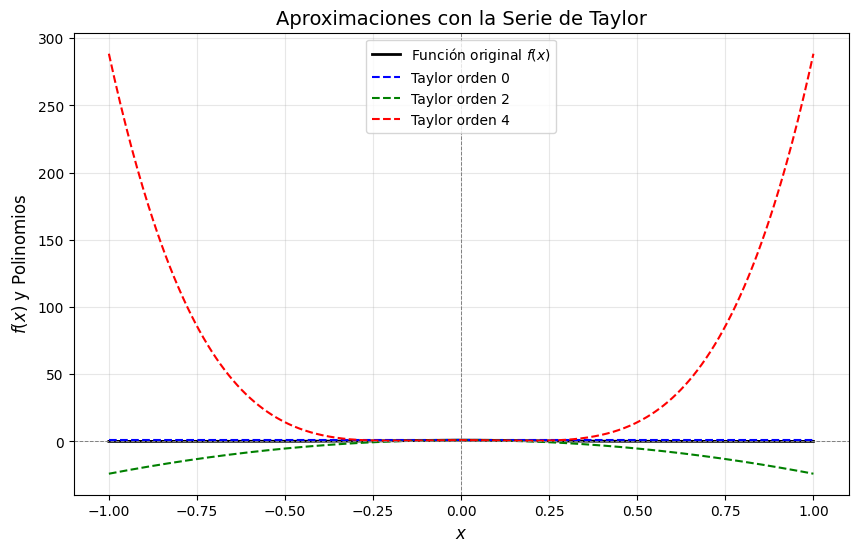
\includegraphics{Deber6_files/figure-pdf/cell-2-output-1.png}

\subsection{2. Serie de Taylor para arctan(x) centrada en
x=1}\label{serie-de-taylor-para-arctanx-centrada-en-x1}

\subsubsection{\texorpdfstring{Paso 1: Serie de Taylor para
\(f(x) = \arctan(x)\) en
\(x_0 = 1\)}{Paso 1: Serie de Taylor para f(x) = \textbackslash arctan(x) en x\_0 = 1}}\label{paso-1-serie-de-taylor-para-fx-arctanx-en-x_0-1}

La fórmula general de la serie de Taylor es:

\[
f(x) \approx f(x_0) + f'(x_0)(x - x_0) + \frac{f''(x_0)}{2!}(x - x_0)^2 + \frac{f^{(3)}(x_0)}{3!}(x - x_0)^3 + \dots
\]

Para \(f(x) = \arctan(x)\), calculamos las derivadas en \(x_0 = 1\):

\begin{center}\rule{0.5\linewidth}{0.5pt}\end{center}

\paragraph{Primera derivada:}\label{primera-derivada}

\[
f'(x) = \frac{1}{1 + x^2}, \quad f'(1) = \frac{1}{1 + 1^2} = \frac{1}{2}.
\]

\begin{center}\rule{0.5\linewidth}{0.5pt}\end{center}

\paragraph{Segunda derivada:}\label{segunda-derivada}

\[
f''(x) = \frac{-2x}{(1 + x^2)^2}, \quad f''(1) = \frac{-2(1)}{(1 + 1^2)^2} = \frac{-2}{4} = -\frac{1}{2}.
\]

\begin{center}\rule{0.5\linewidth}{0.5pt}\end{center}

\paragraph{Tercera derivada:}\label{tercera-derivada}

\[
f^{(3)}(x) = \frac{6x^2 - 2}{(1 + x^2)^3}, \quad f^{(3)}(1) = \frac{6(1)^2 - 2}{(1 + 1^2)^3} = \frac{6 - 2}{8} = \frac{4}{8} = \frac{1}{2}.
\]

\begin{center}\rule{0.5\linewidth}{0.5pt}\end{center}

\paragraph{Cuarta derivada:}\label{cuarta-derivada}

\[
f^{(4)}(x) = \frac{-24x(x^2 - 1)}{(1 + x^2)^4}, \quad f^{(4)}(1) = \frac{-24(1)(1^2 - 1)}{(1 + 1^2)^4} = 0.
\]

\begin{center}\rule{0.5\linewidth}{0.5pt}\end{center}

\paragraph{Sustituyendo en la fórmula de
Taylor:}\label{sustituyendo-en-la-fuxf3rmula-de-taylor}

\[
f(x) \approx \arctan(1) + \frac{1}{2}(x - 1) - \frac{1}{4}(x - 1)^2 + \frac{1}{12}(x - 1)^3.
\]

\begin{Shaded}
\begin{Highlighting}[]
\ImportTok{import}\NormalTok{ numpy }\ImportTok{as}\NormalTok{ np}
\ImportTok{import}\NormalTok{ matplotlib.pyplot }\ImportTok{as}\NormalTok{ plt}

\CommentTok{\# Función original}
\KeywordTok{def}\NormalTok{ f(x):}
    \ControlFlowTok{return}\NormalTok{ np.arctan(x)}

\CommentTok{\# Polinomios de Taylor}
\KeywordTok{def}\NormalTok{ taylor\_order\_0(x):}
    \ControlFlowTok{return}\NormalTok{ np.full\_like(x, np.pi }\OperatorTok{/} \DecValTok{4}\NormalTok{)  }\CommentTok{\# Arreglo constante}

\KeywordTok{def}\NormalTok{ taylor\_order\_1(x):}
    \ControlFlowTok{return}\NormalTok{ np.pi }\OperatorTok{/} \DecValTok{4} \OperatorTok{+}\NormalTok{ (}\DecValTok{1} \OperatorTok{/} \DecValTok{2}\NormalTok{) }\OperatorTok{*}\NormalTok{ (x }\OperatorTok{{-}} \DecValTok{1}\NormalTok{)}

\KeywordTok{def}\NormalTok{ taylor\_order\_2(x):}
    \ControlFlowTok{return}\NormalTok{ np.pi }\OperatorTok{/} \DecValTok{4} \OperatorTok{+}\NormalTok{ (}\DecValTok{1} \OperatorTok{/} \DecValTok{2}\NormalTok{) }\OperatorTok{*}\NormalTok{ (x }\OperatorTok{{-}} \DecValTok{1}\NormalTok{) }\OperatorTok{{-}}\NormalTok{ (}\DecValTok{1} \OperatorTok{/} \DecValTok{4}\NormalTok{) }\OperatorTok{*}\NormalTok{ (x }\OperatorTok{{-}} \DecValTok{1}\NormalTok{)}\OperatorTok{**}\DecValTok{2}

\KeywordTok{def}\NormalTok{ taylor\_order\_3(x):}
    \ControlFlowTok{return}\NormalTok{ np.pi }\OperatorTok{/} \DecValTok{4} \OperatorTok{+}\NormalTok{ (}\DecValTok{1} \OperatorTok{/} \DecValTok{2}\NormalTok{) }\OperatorTok{*}\NormalTok{ (x }\OperatorTok{{-}} \DecValTok{1}\NormalTok{) }\OperatorTok{{-}}\NormalTok{ (}\DecValTok{1} \OperatorTok{/} \DecValTok{4}\NormalTok{) }\OperatorTok{*}\NormalTok{ (x }\OperatorTok{{-}} \DecValTok{1}\NormalTok{)}\OperatorTok{**}\DecValTok{2} \OperatorTok{+}\NormalTok{ (}\DecValTok{1} \OperatorTok{/} \DecValTok{12}\NormalTok{) }\OperatorTok{*}\NormalTok{ (x }\OperatorTok{{-}} \DecValTok{1}\NormalTok{)}\OperatorTok{**}\DecValTok{3}

\CommentTok{\# Rango de x y puntos}
\NormalTok{x }\OperatorTok{=}\NormalTok{ np.linspace(}\DecValTok{0}\NormalTok{, }\DecValTok{2}\NormalTok{, }\DecValTok{500}\NormalTok{)  }\CommentTok{\# Rango [0, 2]}
\NormalTok{y }\OperatorTok{=}\NormalTok{ f(x)}

\CommentTok{\# Calcular aproximaciones}
\NormalTok{y\_taylor\_0 }\OperatorTok{=}\NormalTok{ taylor\_order\_0(x)}
\NormalTok{y\_taylor\_1 }\OperatorTok{=}\NormalTok{ taylor\_order\_1(x)}
\NormalTok{y\_taylor\_2 }\OperatorTok{=}\NormalTok{ taylor\_order\_2(x)}
\NormalTok{y\_taylor\_3 }\OperatorTok{=}\NormalTok{ taylor\_order\_3(x)}

\CommentTok{\# Gráficas}
\NormalTok{plt.figure(figsize}\OperatorTok{=}\NormalTok{(}\DecValTok{10}\NormalTok{, }\DecValTok{6}\NormalTok{))}
\NormalTok{plt.plot(x, y, label}\OperatorTok{=}\StringTok{\textquotesingle{}Función original $f(x) = }\CharTok{\textbackslash{}\textbackslash{}}\StringTok{arctan(x)$\textquotesingle{}}\NormalTok{, color}\OperatorTok{=}\StringTok{\textquotesingle{}black\textquotesingle{}}\NormalTok{, linewidth}\OperatorTok{=}\DecValTok{2}\NormalTok{)}
\NormalTok{plt.plot(x, y\_taylor\_0, label}\OperatorTok{=}\StringTok{\textquotesingle{}Taylor orden 0\textquotesingle{}}\NormalTok{, linestyle}\OperatorTok{=}\StringTok{\textquotesingle{}{-}{-}\textquotesingle{}}\NormalTok{, color}\OperatorTok{=}\StringTok{\textquotesingle{}blue\textquotesingle{}}\NormalTok{)}
\NormalTok{plt.plot(x, y\_taylor\_1, label}\OperatorTok{=}\StringTok{\textquotesingle{}Taylor orden 1\textquotesingle{}}\NormalTok{, linestyle}\OperatorTok{=}\StringTok{\textquotesingle{}{-}{-}\textquotesingle{}}\NormalTok{, color}\OperatorTok{=}\StringTok{\textquotesingle{}green\textquotesingle{}}\NormalTok{)}
\NormalTok{plt.plot(x, y\_taylor\_2, label}\OperatorTok{=}\StringTok{\textquotesingle{}Taylor orden 2\textquotesingle{}}\NormalTok{, linestyle}\OperatorTok{=}\StringTok{\textquotesingle{}{-}{-}\textquotesingle{}}\NormalTok{, color}\OperatorTok{=}\StringTok{\textquotesingle{}red\textquotesingle{}}\NormalTok{)}
\NormalTok{plt.plot(x, y\_taylor\_3, label}\OperatorTok{=}\StringTok{\textquotesingle{}Taylor orden 3\textquotesingle{}}\NormalTok{, linestyle}\OperatorTok{=}\StringTok{\textquotesingle{}{-}{-}\textquotesingle{}}\NormalTok{, color}\OperatorTok{=}\StringTok{\textquotesingle{}purple\textquotesingle{}}\NormalTok{)}

\CommentTok{\# Personalización del gráfico}
\NormalTok{plt.title(}\StringTok{\textquotesingle{}Aproximaciones con la Serie de Taylor para $}\CharTok{\textbackslash{}\textbackslash{}}\StringTok{arctan(x)$ en $x\_0 = 1$\textquotesingle{}}\NormalTok{, fontsize}\OperatorTok{=}\DecValTok{14}\NormalTok{)}
\NormalTok{plt.xlabel(}\StringTok{\textquotesingle{}$x$\textquotesingle{}}\NormalTok{, fontsize}\OperatorTok{=}\DecValTok{12}\NormalTok{)}
\NormalTok{plt.ylabel(}\StringTok{\textquotesingle{}$f(x)$ y Polinomios\textquotesingle{}}\NormalTok{, fontsize}\OperatorTok{=}\DecValTok{12}\NormalTok{)}
\NormalTok{plt.axhline(}\DecValTok{0}\NormalTok{, color}\OperatorTok{=}\StringTok{\textquotesingle{}gray\textquotesingle{}}\NormalTok{, linestyle}\OperatorTok{=}\StringTok{\textquotesingle{}{-}{-}\textquotesingle{}}\NormalTok{, linewidth}\OperatorTok{=}\FloatTok{0.7}\NormalTok{)}
\NormalTok{plt.axvline(}\DecValTok{0}\NormalTok{, color}\OperatorTok{=}\StringTok{\textquotesingle{}gray\textquotesingle{}}\NormalTok{, linestyle}\OperatorTok{=}\StringTok{\textquotesingle{}{-}{-}\textquotesingle{}}\NormalTok{, linewidth}\OperatorTok{=}\FloatTok{0.7}\NormalTok{)}
\NormalTok{plt.legend(fontsize}\OperatorTok{=}\DecValTok{10}\NormalTok{)}
\NormalTok{plt.grid(alpha}\OperatorTok{=}\FloatTok{0.3}\NormalTok{)}
\NormalTok{plt.show()}
\end{Highlighting}
\end{Shaded}

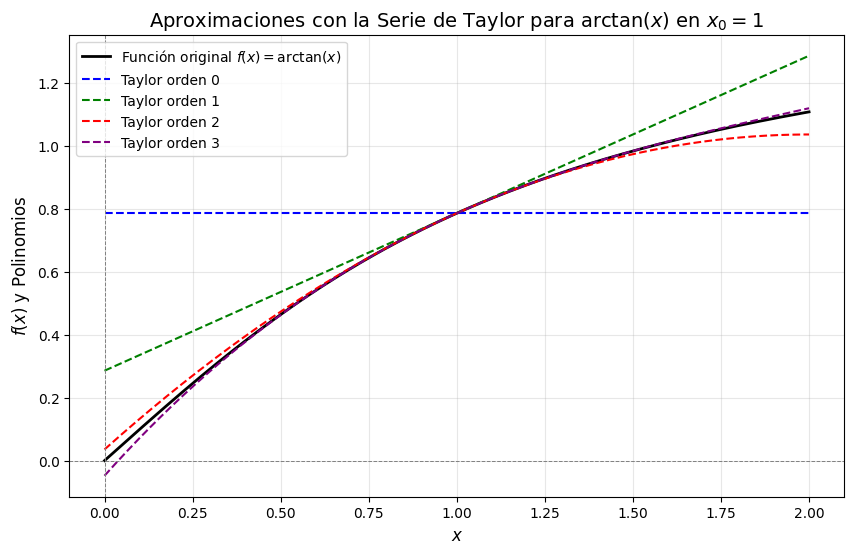
\includegraphics{Deber6_files/figure-pdf/cell-3-output-1.png}

\subsection{Polinomios de Lagrange}\label{polinomios-de-lagrange}

\paragraph{Función 1:}\label{funciuxf3n-1-1}

\[
f(x) = \frac{1}{25x^2 + 1}, \quad x_0 = 0
\]

\begin{Shaded}
\begin{Highlighting}[]
\ImportTok{import}\NormalTok{ numpy }\ImportTok{as}\NormalTok{ np}
\ImportTok{import}\NormalTok{ matplotlib.pyplot }\ImportTok{as}\NormalTok{ plt}

\CommentTok{\# Definimos los puntos}
\NormalTok{x\_points }\OperatorTok{=}\NormalTok{ np.array([}\OperatorTok{{-}}\DecValTok{1}\NormalTok{, }\DecValTok{0}\NormalTok{, }\DecValTok{1}\NormalTok{])}
\NormalTok{y\_points }\OperatorTok{=}\NormalTok{ np.array([}\DecValTok{1}\OperatorTok{/}\DecValTok{26}\NormalTok{, }\DecValTok{1}\NormalTok{, }\DecValTok{1}\OperatorTok{/}\DecValTok{26}\NormalTok{])}

\CommentTok{\# Función de Lagrange}
\KeywordTok{def}\NormalTok{ lagrange\_interpolation(x, x\_points, y\_points):}
\NormalTok{    total\_sum }\OperatorTok{=} \DecValTok{0}
\NormalTok{    n }\OperatorTok{=} \BuiltInTok{len}\NormalTok{(x\_points)}
    \ControlFlowTok{for}\NormalTok{ i }\KeywordTok{in} \BuiltInTok{range}\NormalTok{(n):}
\NormalTok{        xi, yi }\OperatorTok{=}\NormalTok{ x\_points[i], y\_points[i]}
\NormalTok{        product }\OperatorTok{=}\NormalTok{ yi}
        \ControlFlowTok{for}\NormalTok{ j }\KeywordTok{in} \BuiltInTok{range}\NormalTok{(n):}
            \ControlFlowTok{if}\NormalTok{ i }\OperatorTok{!=}\NormalTok{ j:}
\NormalTok{                xj }\OperatorTok{=}\NormalTok{ x\_points[j]}
\NormalTok{                product }\OperatorTok{*=}\NormalTok{ (x }\OperatorTok{{-}}\NormalTok{ xj) }\OperatorTok{/}\NormalTok{ (xi }\OperatorTok{{-}}\NormalTok{ xj)}
\NormalTok{        total\_sum }\OperatorTok{+=}\NormalTok{ product}
    \ControlFlowTok{return}\NormalTok{ total\_sum}

\CommentTok{\# Rango de x y puntos}
\NormalTok{x }\OperatorTok{=}\NormalTok{ np.linspace(}\OperatorTok{{-}}\FloatTok{1.5}\NormalTok{, }\FloatTok{1.5}\NormalTok{, }\DecValTok{500}\NormalTok{)}
\NormalTok{y\_lagrange }\OperatorTok{=}\NormalTok{ lagrange\_interpolation(x, x\_points, y\_points)}

\CommentTok{\# Gráfica}
\NormalTok{plt.figure(figsize}\OperatorTok{=}\NormalTok{(}\DecValTok{10}\NormalTok{, }\DecValTok{6}\NormalTok{))}
\NormalTok{plt.plot(x, y\_lagrange, label}\OperatorTok{=}\StringTok{\textquotesingle{}Polinomio de Lagrange\textquotesingle{}}\NormalTok{, color}\OperatorTok{=}\StringTok{\textquotesingle{}blue\textquotesingle{}}\NormalTok{)}
\NormalTok{plt.scatter(x\_points, y\_points, color}\OperatorTok{=}\StringTok{\textquotesingle{}red\textquotesingle{}}\NormalTok{, zorder}\OperatorTok{=}\DecValTok{5}\NormalTok{)  }\CommentTok{\# Puntos dados}

\CommentTok{\# Personalización del gráfico}
\NormalTok{plt.title(}\StringTok{\textquotesingle{}Aproximación con el Polinomio de Lagrange\textquotesingle{}}\NormalTok{, fontsize}\OperatorTok{=}\DecValTok{14}\NormalTok{)}
\NormalTok{plt.xlabel(}\StringTok{\textquotesingle{}$x$\textquotesingle{}}\NormalTok{, fontsize}\OperatorTok{=}\DecValTok{12}\NormalTok{)}
\NormalTok{plt.ylabel(}\StringTok{\textquotesingle{}$f(x)$\textquotesingle{}}\NormalTok{, fontsize}\OperatorTok{=}\DecValTok{12}\NormalTok{)}
\NormalTok{plt.axhline(}\DecValTok{0}\NormalTok{, color}\OperatorTok{=}\StringTok{\textquotesingle{}gray\textquotesingle{}}\NormalTok{, linestyle}\OperatorTok{=}\StringTok{\textquotesingle{}{-}{-}\textquotesingle{}}\NormalTok{, linewidth}\OperatorTok{=}\FloatTok{0.7}\NormalTok{)}
\NormalTok{plt.axvline(}\DecValTok{0}\NormalTok{, color}\OperatorTok{=}\StringTok{\textquotesingle{}gray\textquotesingle{}}\NormalTok{, linestyle}\OperatorTok{=}\StringTok{\textquotesingle{}{-}{-}\textquotesingle{}}\NormalTok{, linewidth}\OperatorTok{=}\FloatTok{0.7}\NormalTok{)}
\NormalTok{plt.legend(fontsize}\OperatorTok{=}\DecValTok{10}\NormalTok{)}
\NormalTok{plt.grid(alpha}\OperatorTok{=}\FloatTok{0.3}\NormalTok{)}
\NormalTok{plt.show()}
\CommentTok{\# Graficar la función original junto con el polinomio de Lagrange}
\NormalTok{y\_original }\OperatorTok{=} \DecValTok{1} \OperatorTok{/}\NormalTok{ (}\DecValTok{25} \OperatorTok{*}\NormalTok{ x}\OperatorTok{**}\DecValTok{2} \OperatorTok{+} \DecValTok{1}\NormalTok{)}

\NormalTok{plt.figure(figsize}\OperatorTok{=}\NormalTok{(}\DecValTok{10}\NormalTok{, }\DecValTok{6}\NormalTok{))}
\NormalTok{plt.plot(x, y\_original, label}\OperatorTok{=}\StringTok{\textquotesingle{}Función original $f(x)$\textquotesingle{}}\NormalTok{, color}\OperatorTok{=}\StringTok{\textquotesingle{}black\textquotesingle{}}\NormalTok{, linewidth}\OperatorTok{=}\DecValTok{2}\NormalTok{)}
\NormalTok{plt.plot(x, y\_lagrange, label}\OperatorTok{=}\StringTok{\textquotesingle{}Polinomio de Lagrange\textquotesingle{}}\NormalTok{, color}\OperatorTok{=}\StringTok{\textquotesingle{}blue\textquotesingle{}}\NormalTok{, linestyle}\OperatorTok{=}\StringTok{\textquotesingle{}{-}{-}\textquotesingle{}}\NormalTok{)}
\NormalTok{plt.scatter(x\_points, y\_points, color}\OperatorTok{=}\StringTok{\textquotesingle{}red\textquotesingle{}}\NormalTok{, zorder}\OperatorTok{=}\DecValTok{5}\NormalTok{)  }\CommentTok{\# Puntos dados}

\CommentTok{\# Personalización del gráfico}
\NormalTok{plt.title(}\StringTok{\textquotesingle{}Función original y Polinomio de Lagrange\textquotesingle{}}\NormalTok{, fontsize}\OperatorTok{=}\DecValTok{14}\NormalTok{)}
\NormalTok{plt.xlabel(}\StringTok{\textquotesingle{}$x$\textquotesingle{}}\NormalTok{, fontsize}\OperatorTok{=}\DecValTok{12}\NormalTok{)}
\NormalTok{plt.ylabel(}\StringTok{\textquotesingle{}$f(x)$\textquotesingle{}}\NormalTok{, fontsize}\OperatorTok{=}\DecValTok{12}\NormalTok{)}
\NormalTok{plt.axhline(}\DecValTok{0}\NormalTok{, color}\OperatorTok{=}\StringTok{\textquotesingle{}gray\textquotesingle{}}\NormalTok{, linestyle}\OperatorTok{=}\StringTok{\textquotesingle{}{-}{-}\textquotesingle{}}\NormalTok{, linewidth}\OperatorTok{=}\FloatTok{0.7}\NormalTok{)}
\NormalTok{plt.axvline(}\DecValTok{0}\NormalTok{, color}\OperatorTok{=}\StringTok{\textquotesingle{}gray\textquotesingle{}}\NormalTok{, linestyle}\OperatorTok{=}\StringTok{\textquotesingle{}{-}{-}\textquotesingle{}}\NormalTok{, linewidth}\OperatorTok{=}\FloatTok{0.7}\NormalTok{)}
\NormalTok{plt.legend(fontsize}\OperatorTok{=}\DecValTok{10}\NormalTok{)}
\NormalTok{plt.grid(alpha}\OperatorTok{=}\FloatTok{0.3}\NormalTok{)}
\NormalTok{plt.show()}
\end{Highlighting}
\end{Shaded}

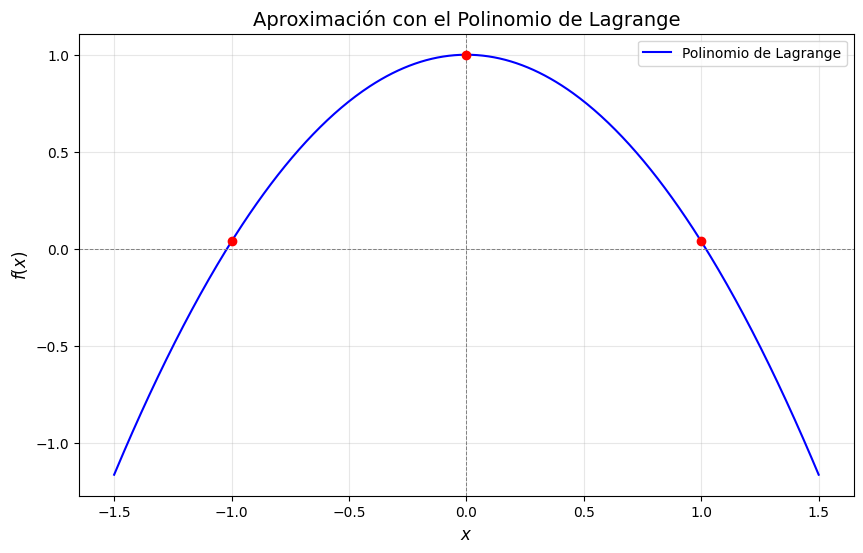
\includegraphics{Deber6_files/figure-pdf/cell-4-output-1.png}

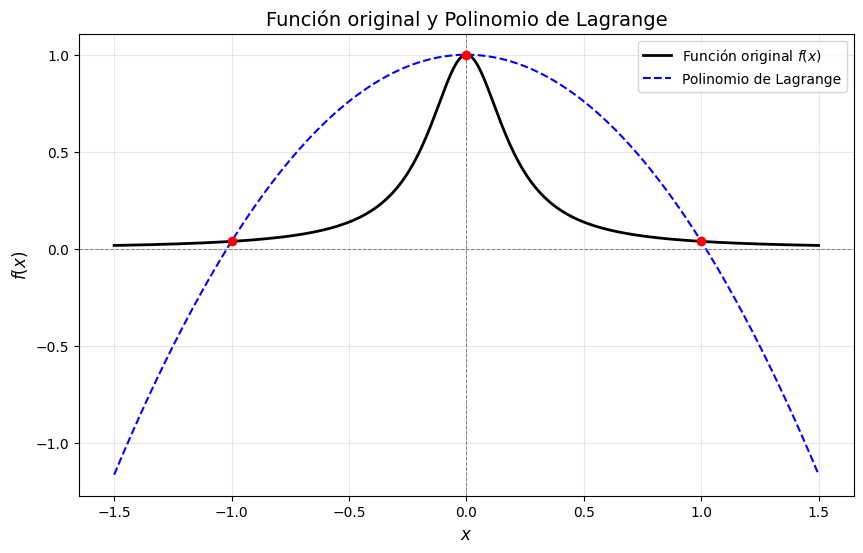
\includegraphics{Deber6_files/figure-pdf/cell-4-output-2.png}

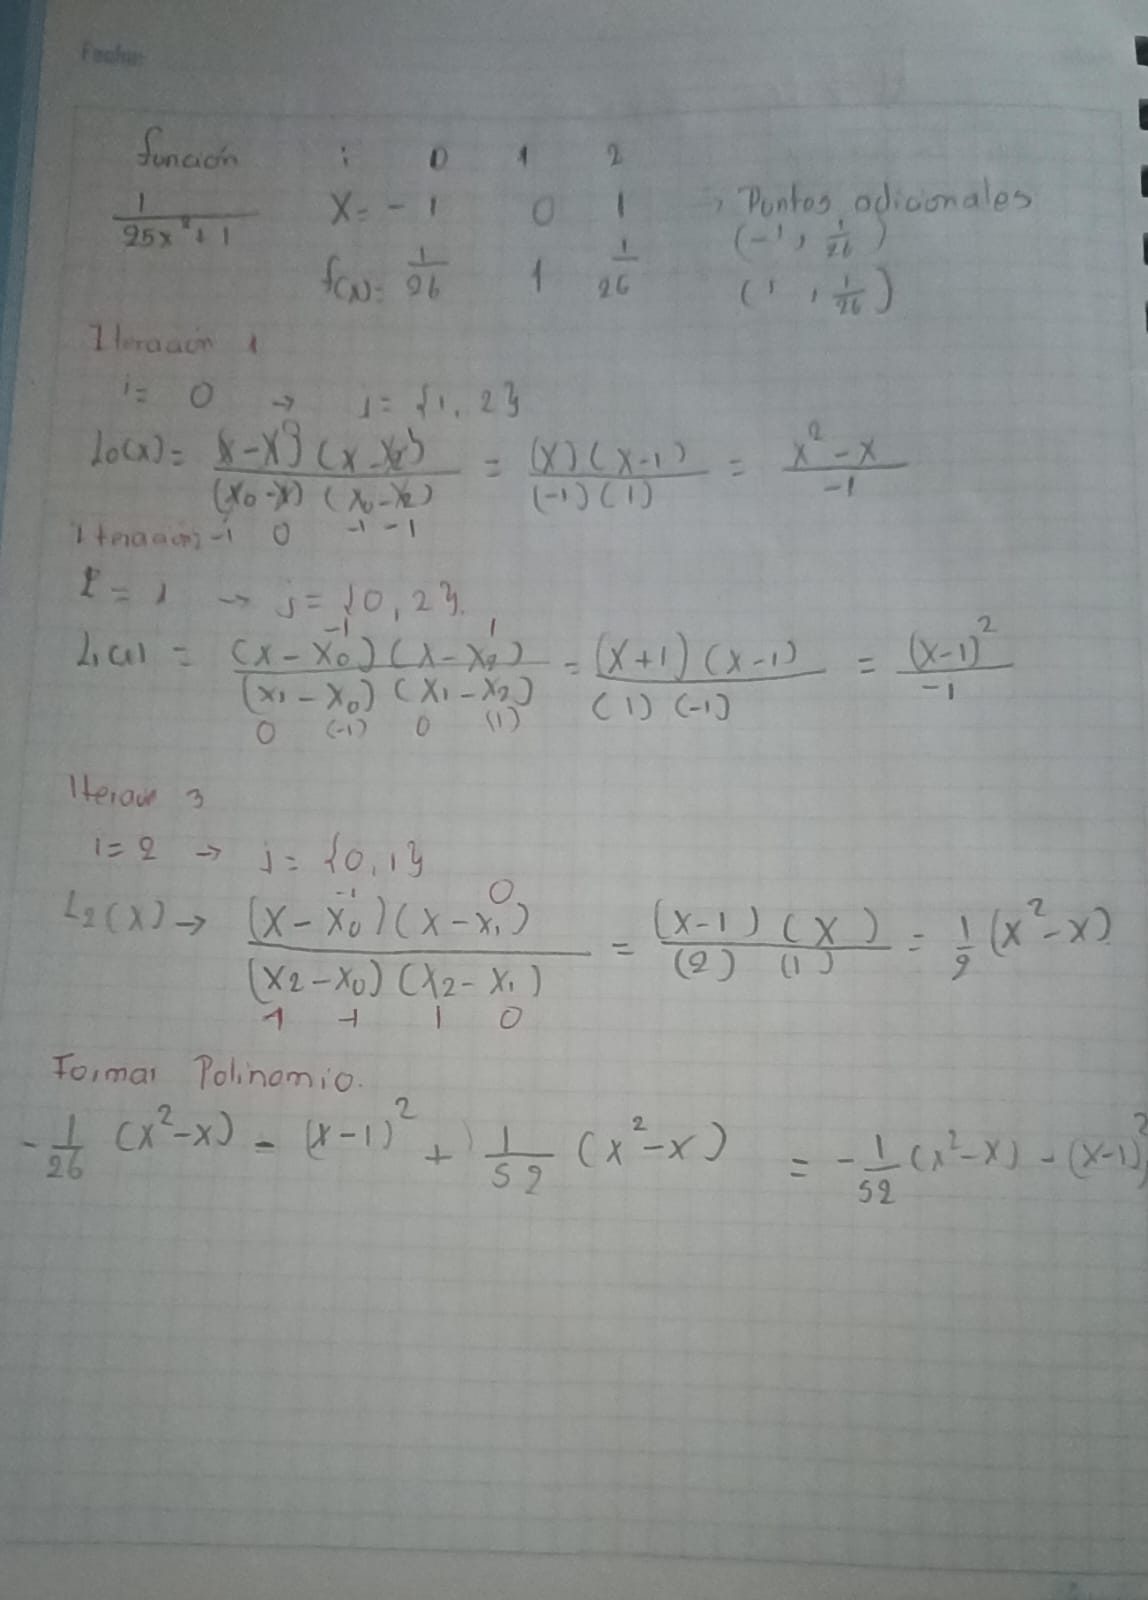
\includegraphics{ejer1.jpeg}

\paragraph{Función 2:}\label{funciuxf3n-2}

\[
f(x) = \arctan(x), \quad x_0 = 1
\]

\begin{center}\rule{0.5\linewidth}{0.5pt}\end{center}

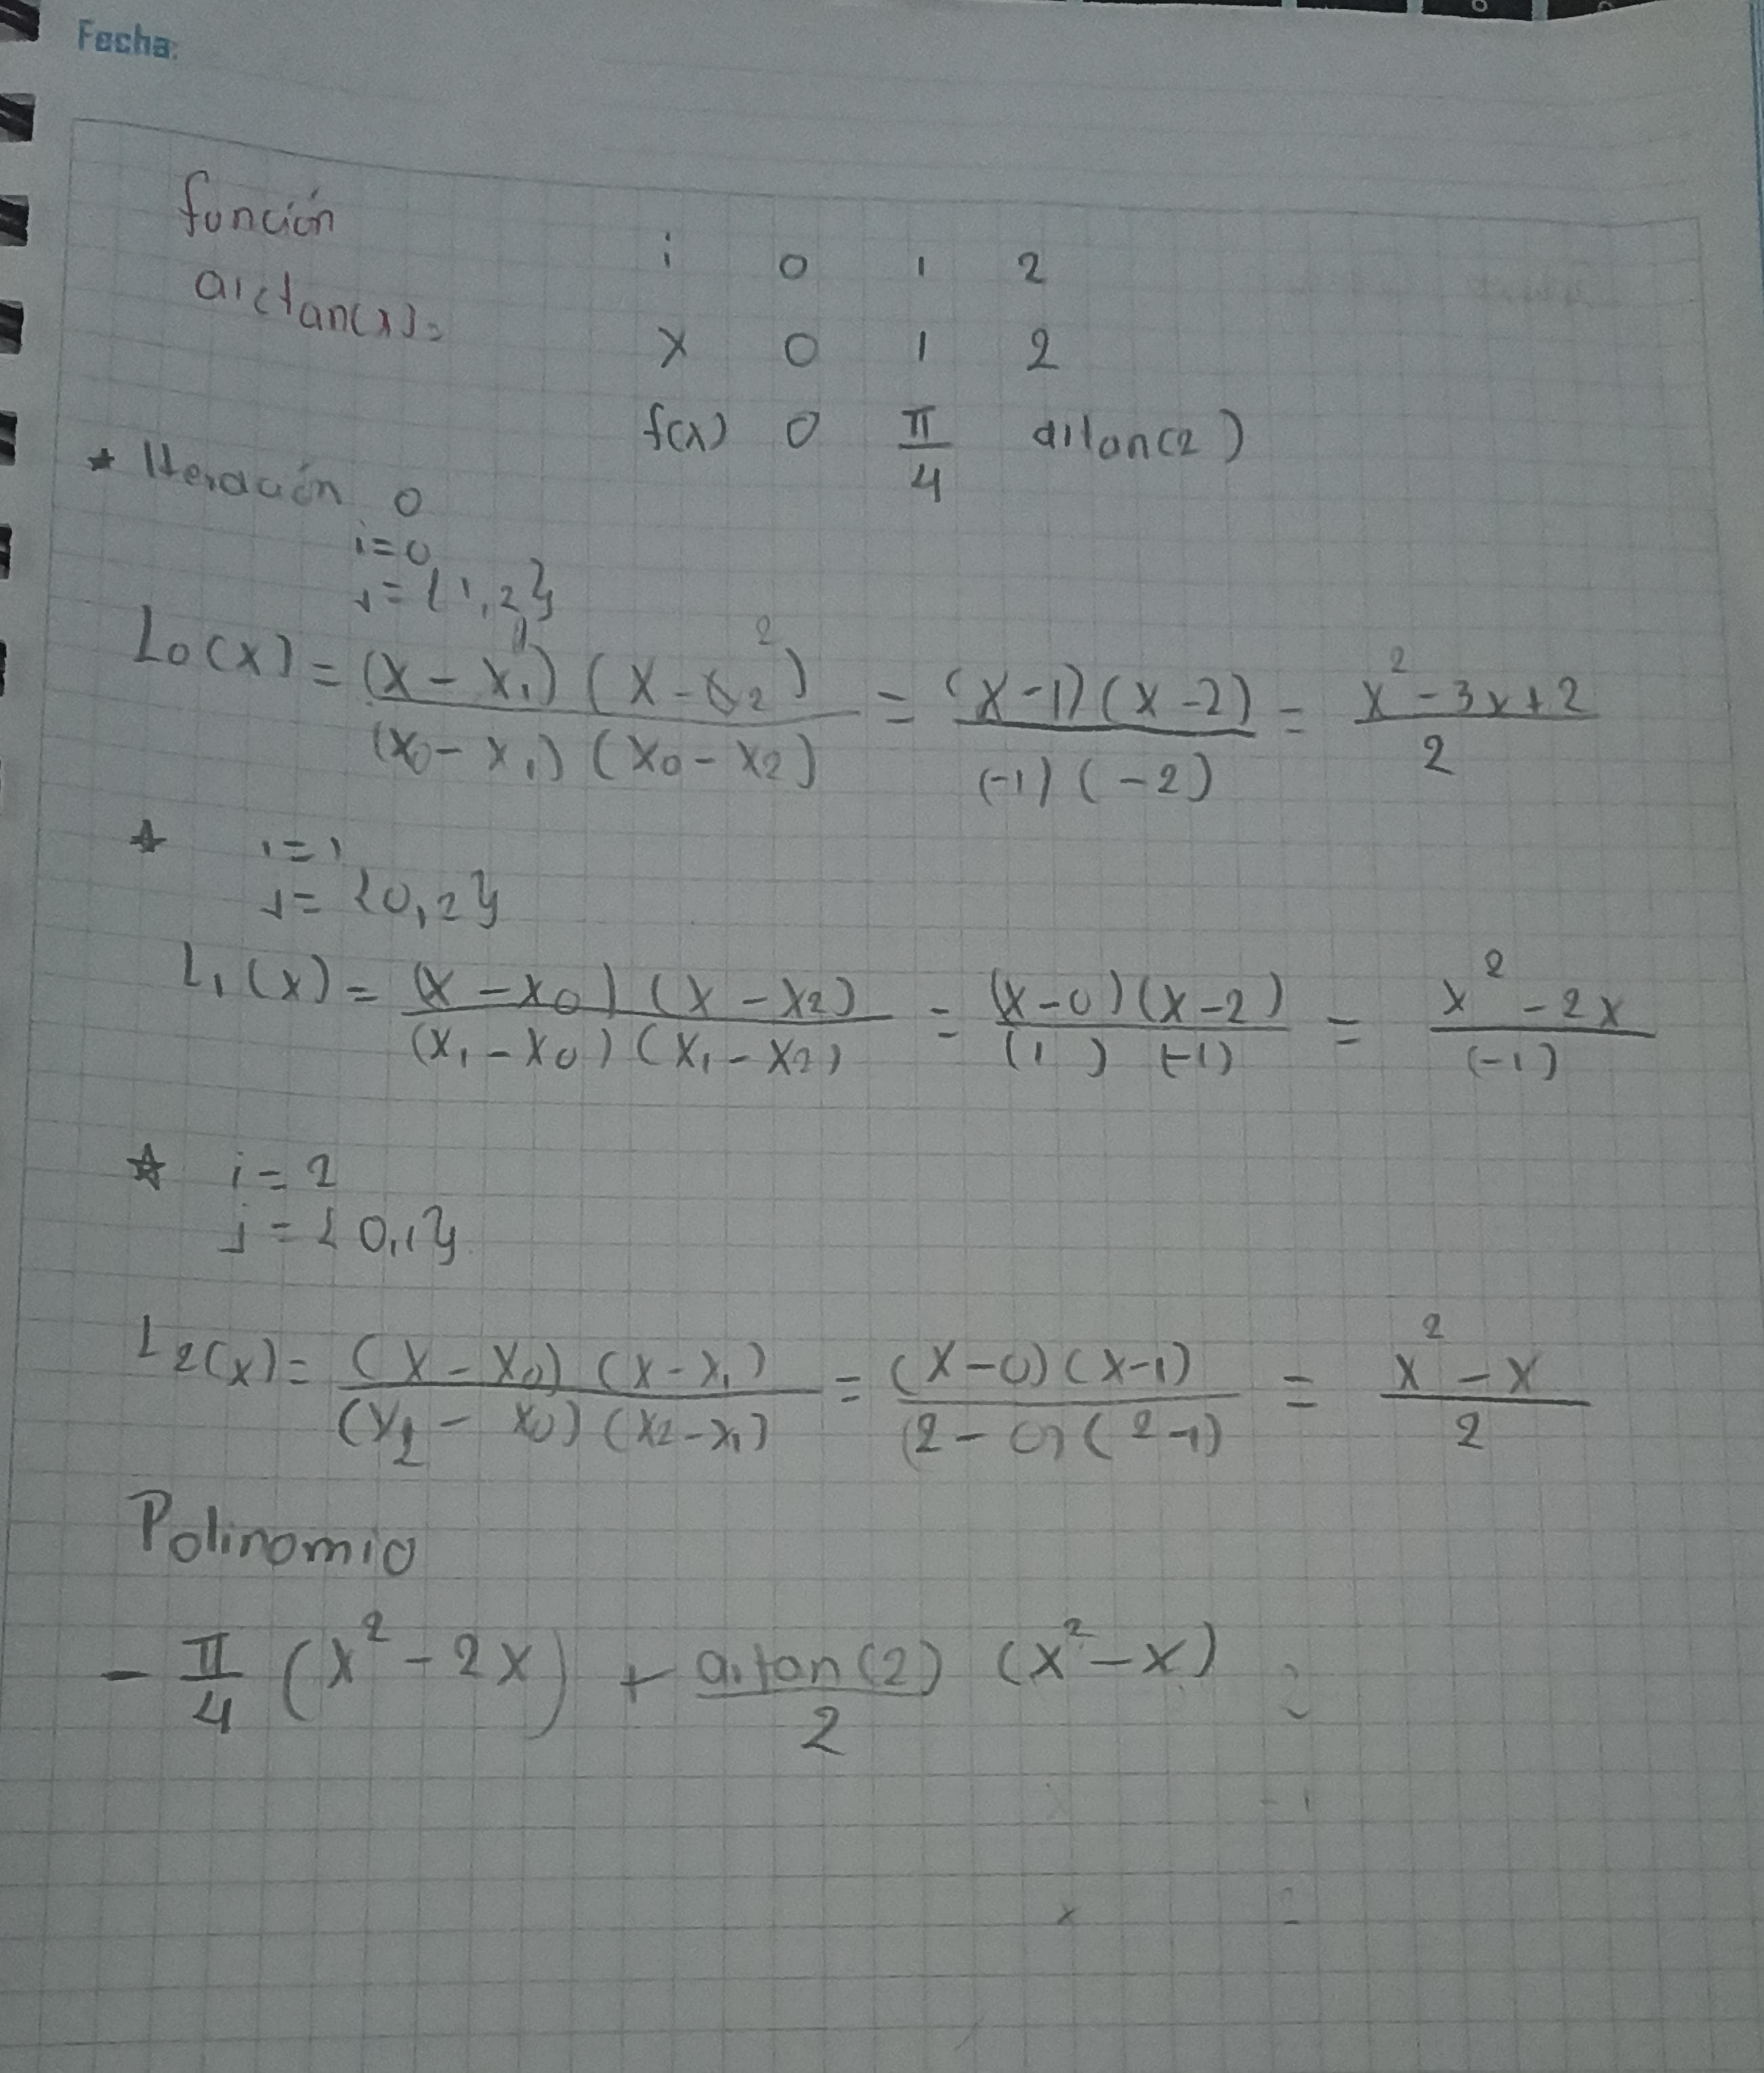
\includegraphics{EJER2V.jpeg}

\subsection{Grafica}\label{grafica}

\begin{Shaded}
\begin{Highlighting}[]
\CommentTok{\# Definimos los puntos para la función 2}
\NormalTok{x\_points\_func2 }\OperatorTok{=}\NormalTok{ np.array([}\DecValTok{0}\NormalTok{, }\DecValTok{1}\NormalTok{, }\DecValTok{2}\NormalTok{])}
\NormalTok{y\_points\_func2 }\OperatorTok{=}\NormalTok{ np.array([}\DecValTok{0}\NormalTok{, np.pi}\OperatorTok{/}\DecValTok{4}\NormalTok{, np.arctan(}\DecValTok{2}\NormalTok{)])}

\CommentTok{\# Función de Lagrange para la función 2}
\KeywordTok{def}\NormalTok{ lagrange\_interpolation\_func2(x, x\_points, y\_points):}
\NormalTok{    total\_sum }\OperatorTok{=} \DecValTok{0}
\NormalTok{    n }\OperatorTok{=} \BuiltInTok{len}\NormalTok{(x\_points)}
    \ControlFlowTok{for}\NormalTok{ i }\KeywordTok{in} \BuiltInTok{range}\NormalTok{(n):}
\NormalTok{        xi, yi }\OperatorTok{=}\NormalTok{ x\_points[i], y\_points[i]}
\NormalTok{        product }\OperatorTok{=}\NormalTok{ yi}
        \ControlFlowTok{for}\NormalTok{ j }\KeywordTok{in} \BuiltInTok{range}\NormalTok{(n):}
            \ControlFlowTok{if}\NormalTok{ i }\OperatorTok{!=}\NormalTok{ j:}
\NormalTok{                xj }\OperatorTok{=}\NormalTok{ x\_points[j]}
\NormalTok{                product }\OperatorTok{*=}\NormalTok{ (x }\OperatorTok{{-}}\NormalTok{ xj) }\OperatorTok{/}\NormalTok{ (xi }\OperatorTok{{-}}\NormalTok{ xj)}
\NormalTok{        total\_sum }\OperatorTok{+=}\NormalTok{ product}
    \ControlFlowTok{return}\NormalTok{ total\_sum}

\CommentTok{\# Calcular la interpolación de Lagrange para la función 2}
\NormalTok{y\_lagrange\_func2 }\OperatorTok{=}\NormalTok{ lagrange\_interpolation\_func2(x, x\_points\_func2, y\_points\_func2)}

\CommentTok{\# Gráfica de la función original y el polinomio de Lagrange}
\NormalTok{plt.figure(figsize}\OperatorTok{=}\NormalTok{(}\DecValTok{10}\NormalTok{, }\DecValTok{6}\NormalTok{))}
\NormalTok{plt.plot(x, np.arctan(x), label}\OperatorTok{=}\StringTok{\textquotesingle{}Función original $f(x) = }\CharTok{\textbackslash{}\textbackslash{}}\StringTok{arctan(x)$\textquotesingle{}}\NormalTok{, color}\OperatorTok{=}\StringTok{\textquotesingle{}black\textquotesingle{}}\NormalTok{, linewidth}\OperatorTok{=}\DecValTok{2}\NormalTok{)}
\NormalTok{plt.plot(x, y\_lagrange\_func2, label}\OperatorTok{=}\StringTok{\textquotesingle{}Polinomio de Lagrange\textquotesingle{}}\NormalTok{, color}\OperatorTok{=}\StringTok{\textquotesingle{}blue\textquotesingle{}}\NormalTok{, linestyle}\OperatorTok{=}\StringTok{\textquotesingle{}{-}{-}\textquotesingle{}}\NormalTok{)}
\NormalTok{plt.scatter(x\_points\_func2, y\_points\_func2, color}\OperatorTok{=}\StringTok{\textquotesingle{}red\textquotesingle{}}\NormalTok{, zorder}\OperatorTok{=}\DecValTok{5}\NormalTok{)  }\CommentTok{\# Puntos dados}

\CommentTok{\# Personalización del gráfico}
\NormalTok{plt.title(}\StringTok{\textquotesingle{}Función original y Polinomio de Lagrange para $}\CharTok{\textbackslash{}\textbackslash{}}\StringTok{arctan(x)$\textquotesingle{}}\NormalTok{, fontsize}\OperatorTok{=}\DecValTok{14}\NormalTok{)}
\NormalTok{plt.xlabel(}\StringTok{\textquotesingle{}$x$\textquotesingle{}}\NormalTok{, fontsize}\OperatorTok{=}\DecValTok{12}\NormalTok{)}
\NormalTok{plt.ylabel(}\StringTok{\textquotesingle{}$f(x)$\textquotesingle{}}\NormalTok{, fontsize}\OperatorTok{=}\DecValTok{12}\NormalTok{)}
\NormalTok{plt.axhline(}\DecValTok{0}\NormalTok{, color}\OperatorTok{=}\StringTok{\textquotesingle{}gray\textquotesingle{}}\NormalTok{, linestyle}\OperatorTok{=}\StringTok{\textquotesingle{}{-}{-}\textquotesingle{}}\NormalTok{, linewidth}\OperatorTok{=}\FloatTok{0.7}\NormalTok{)}
\NormalTok{plt.axvline(}\DecValTok{0}\NormalTok{, color}\OperatorTok{=}\StringTok{\textquotesingle{}gray\textquotesingle{}}\NormalTok{, linestyle}\OperatorTok{=}\StringTok{\textquotesingle{}{-}{-}\textquotesingle{}}\NormalTok{, linewidth}\OperatorTok{=}\FloatTok{0.7}\NormalTok{)}
\NormalTok{plt.legend(fontsize}\OperatorTok{=}\DecValTok{10}\NormalTok{)}
\NormalTok{plt.grid(alpha}\OperatorTok{=}\FloatTok{0.3}\NormalTok{)}
\NormalTok{plt.show()}
\end{Highlighting}
\end{Shaded}

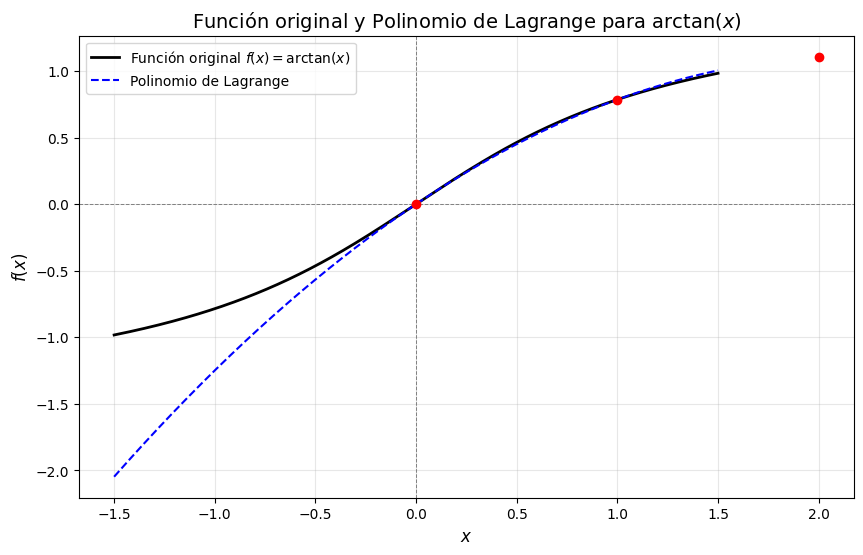
\includegraphics{Deber6_files/figure-pdf/cell-5-output-1.png}




\end{document}
